\documentclass[aspectratio=169,11pt]{beamer}
\usetheme{default}
\usepackage[T1]{fontenc}
\usepackage{lmodern}
\usepackage{booktabs,tikz,xcolor}
\usetikzlibrary{positioning,arrows.meta,fit}
\graphicspath{{../figures/}{../../results/plots/}{../demo/}}
\definecolor{ggblue}{HTML}{2A78D6}
\definecolor{ggorange}{HTML}{EB6834}
\definecolor{gggreen}{HTML}{1BAF7A}
\definecolor{ink2}{HTML}{52514E}
\definecolor{inkdark}{HTML}{1C1E22}
\usefonttheme{professionalfonts}
\setbeamertemplate{navigation symbols}{}
\setbeamercolor{frametitle}{bg=inkdark,fg=white}
\setbeamercolor{title}{fg=inkdark}
\setbeamercolor{subtitle}{fg=ggblue}
\setbeamercolor{structure}{fg=ggblue}
\setbeamercolor{alerted text}{fg=ggorange}
\setbeamercolor{normal text}{fg=inkdark}
\setbeamerfont{frametitle}{size=\large,series=\bfseries}
\setbeamertemplate{frametitle}{\nointerlineskip\begin{beamercolorbox}[wd=\paperwidth,ht=2.6ex,dp=1.4ex,leftskip=1em]{frametitle}
  \usebeamerfont{frametitle}\insertframetitle\end{beamercolorbox}\vspace{0.4em}}
\setbeamertemplate{footline}{\hfill{\scriptsize\color{ink2}\insertframenumber/\inserttotalframenumber}\hspace{1em}\vspace{0.6em}}
\setbeamertemplate{itemize items}[circle]
\setbeamertemplate{enumerate items}[default]
\newcommand{\bignum}[1]{{\Large\bfseries\color{ggblue}#1}}

\title{Processing and Visualising Large DEMs on a Laptop}
\subtitle{GeoGuessers \textbar{} Spatial Informatics, final presentation}
\author{Swayam Goyal (2024111012) \quad Siddharth Choudhary (2024111021)\\Yakkala Viswanadha Kartikeya (2024111033)}
\date{}

\begin{document}
\maketitle

% ------------------------------------------------------------------ problem
\begin{frame}{The problem}
\small
\begin{columns}[T]
\column{0.58\textwidth}
\begin{itemize}
  \item High-resolution DEMs are huge: our 100\,km $\times$ 100\,km Himalayan area at 1\,m is \textbf{10.8 billion
  cells, 43\,GB} as float32.
  \item One laptop: Core Ultra 9 185H (6 performance + 8 efficiency + 2 low-power cores), \textbf{16\,GB RAM},
  RTX 4060 (8\,GB), NVMe SSD.
  \item Users want slope, aspect, hillshade, roughness \ldots\ for whatever they are looking at, \emph{now}.
\end{itemize}
\vspace{6pt}
\textbf{Professor's direction:} process and display \alert{only what is in view}, at the resolution the screen
needs, from a pyramid; choose CPU or GPU by the \alert{measured} bottleneck; integrate with GDAL/QGIS.
\column{0.38\textwidth}
\centering
\bignum{43\,GB}\\[-2pt]{\small grid at 1\,m}\\[10pt]
\bignum{16\,GB}\\[-2pt]{\small RAM}\\[10pt]
\bignum{60 Hz}\\[-2pt]{\small what a map viewer must feel like}
\end{columns}
\end{frame}

\begin{frame}{Research gaps (from our literature review) and questions}
\begin{description}[G1]
  \item[G1] No study reports \textbf{where standard GDAL/QGIS terrain tools stop being practical} on one laptop,
  split by stage (read, compute, CPU$\leftrightarrow$GPU transfer, write, render).
  \item[G2] No study computes \textbf{derivatives on demand from pyramid levels}, or measures the slope error of a
  coarse level against the time it saves.
  \item[G3] Viewshed and terrain distance accuracy (stretch; not done).
\end{description}
\vspace{6pt}
\begin{enumerate}
  \item Where is the real bottleneck, for processing and for display? \hfill \textbf{E1--E4}
  \item What does computing on demand from the pyramid cost in accuracy, and save in time? \hfill \textbf{E5}
  \item Can on-demand computation keep up with continuous pan and zoom? \hfill \textbf{E6}
\end{enumerate}
\end{frame}

\begin{frame}{Data and method}
\begin{columns}[T]
\column{0.45\textwidth}
\centering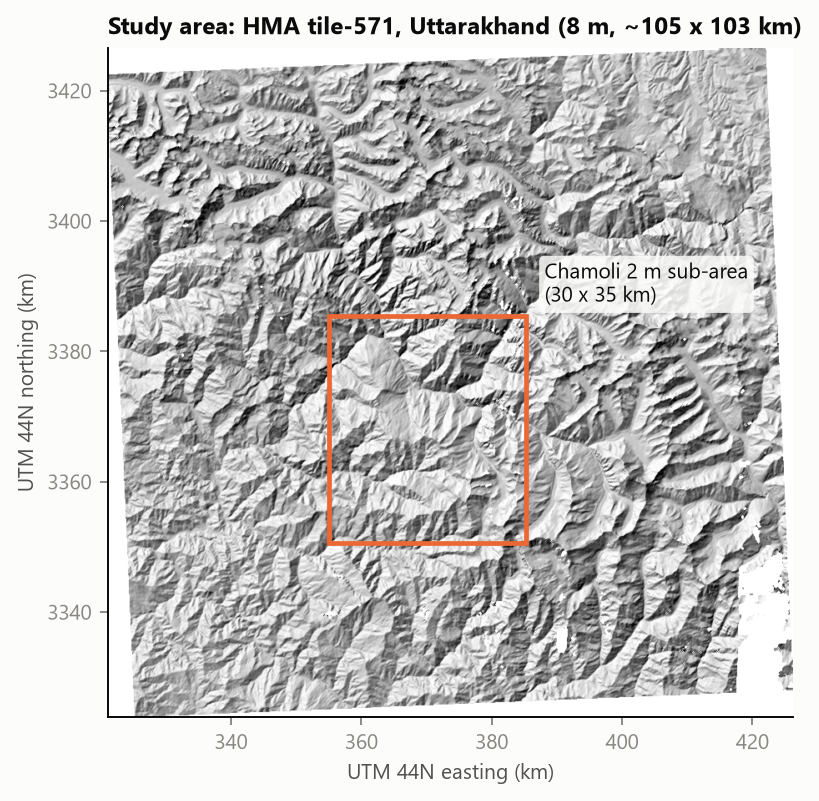
\includegraphics[width=\linewidth,height=0.72\textheight,keepaspectratio]{study_area.png}
\column{0.53\textwidth}
\small
\begin{itemize}
  \item \textbf{Real data:} Chamoli 2\,m (264\,M cells), HMA 8\,m, Copernicus 30/90\,m; UTM 44N.
  \item \textbf{Synthetic 2\,m and 1\,m} versions of the whole area, for timing only (never accuracy).
  \item Cloud-Optimized GeoTIFFs: tiled, ZSTD, overviews = the \textbf{pyramid}.
  \item \textbf{Protocol:} 1 warm-up + 5 measured runs, median and IQR; cold (file cache flushed) and warm; peak
  memory of the measured process; one row per run in \texttt{results/runs.csv}.
  \item Every number in this talk is reproducible from the repository's scripts.
\end{itemize}
\end{columns}
\end{frame}

% ------------------------------------------------------------------ E1
\begin{frame}{E1: standard tools do not fail, they become slow}
\begin{columns}[T]
\column{0.56\textwidth}
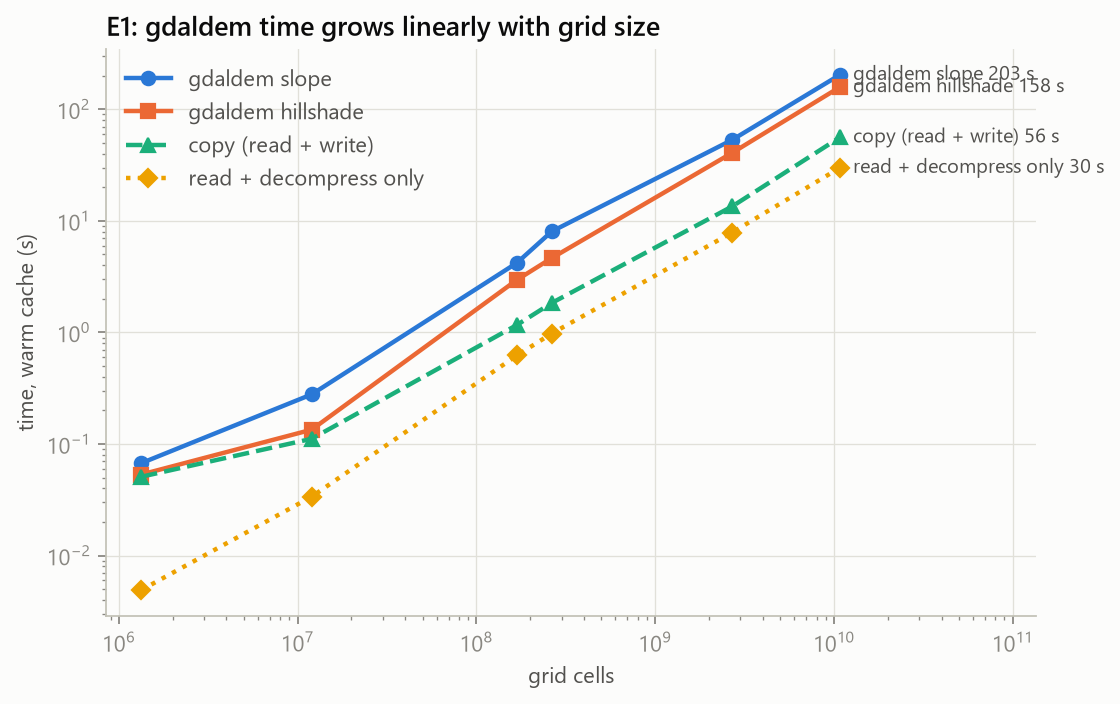
\includegraphics[width=\linewidth]{e1_scaling.png}
\column{0.42\textwidth}
\small
\begin{itemize}
  \item \texttt{gdaldem} streams the grid: peak \textbf{0.87\,GB} even at 1\,m.
  \item Time grows linearly, \textbf{19--25\,ns per cell}: one slope pass over 1\,m takes \textbf{3.5\,min}.
  \item Bottleneck: \alert{one CPU thread computing} (73\% of the time; 1 of 22 threads), not disk (14\%).
  \item File layout matters by up to $\sim$40\%; computation still dominates.
\end{itemize}
\end{columns}
\end{frame}

\begin{frame}{E1: for display, the pyramid is everything}
\begin{columns}[T]
\column{0.56\textwidth}
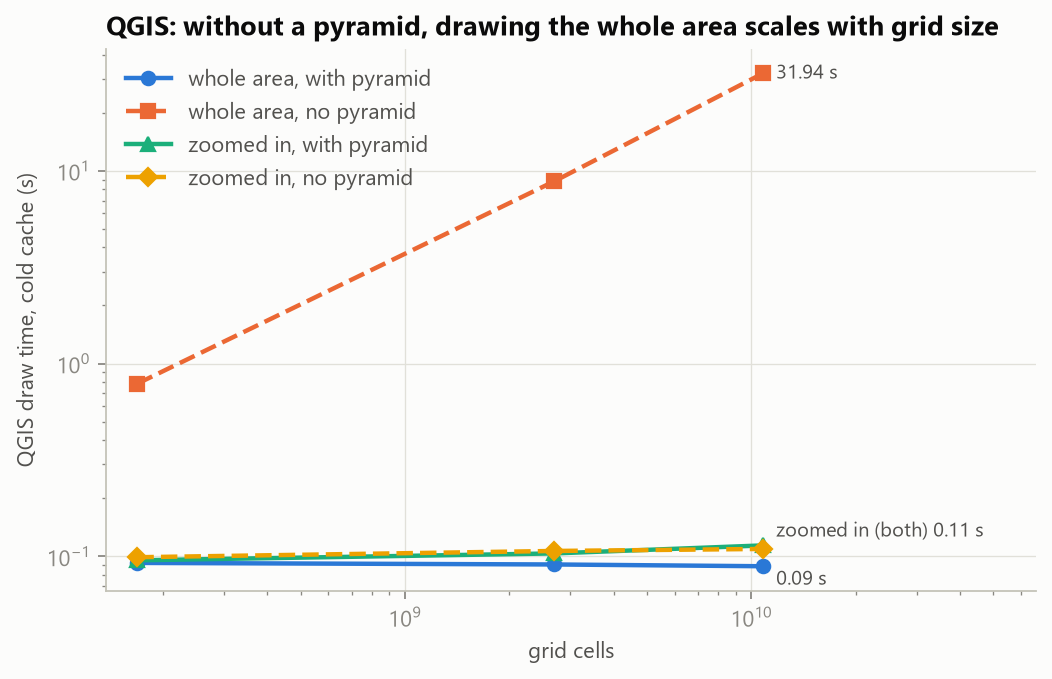
\includegraphics[width=\linewidth]{e1q_render.png}
\column{0.42\textwidth}
\begin{itemize}
  \item QGIS redrawing the whole 1\,m area: \textbf{32\,s} without a pyramid.
  \item With a pyramid: \textbf{0.09\,s} at every resolution.
  \item Display is bound by \alert{reading full-resolution data}; the pyramid removes it.
\end{itemize}
\end{columns}
\end{frame}

% ------------------------------------------------------------------ E3/E4
\begin{frame}{E3: our tiled, parallel CPU engine}
\begin{columns}[T]
\column{0.56\textwidth}
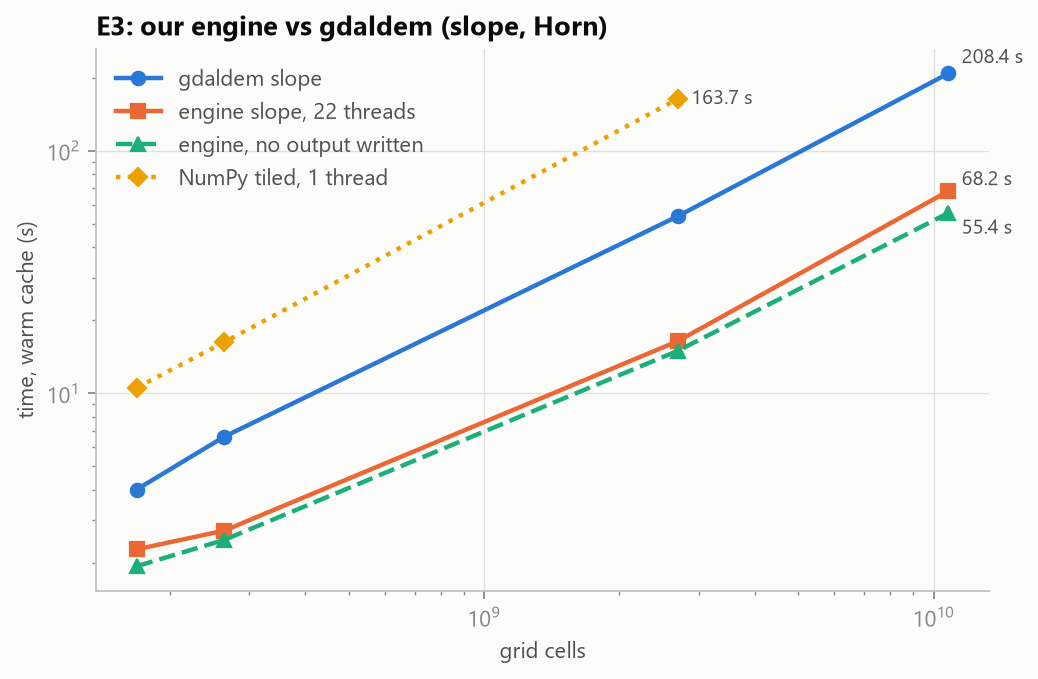
\includegraphics[width=\linewidth]{e3_scaling.png}
\column{0.42\textwidth}
\small
\begin{itemize}
  \item Windows of 2048$^2$ with a 1-cell halo; reader threads $\to$ Numba kernel $\to$ writer.
  \item Slope \textbf{2.1--3.5$\times$ faster than gdaldem} (1\,m: 60\,s vs 208\,s); all 10 gdaldem configurations.
  \item Memory flat at \textbf{1.4\,GB}; whole-grid NumPy runs out of memory from 2\,m synthetic.
  \item Three products in one pass: 3.4--4.2$\times$ fewer seconds than three gdaldem runs.
  \item 12 performance-core threads \alert{beat all 22}.
\end{itemize}
\end{columns}
\end{frame}

\begin{frame}{E4: the GPU computes 50$\times$ faster, the run is 1.0--1.4$\times$ faster}
\begin{columns}[T]
\column{0.56\textwidth}
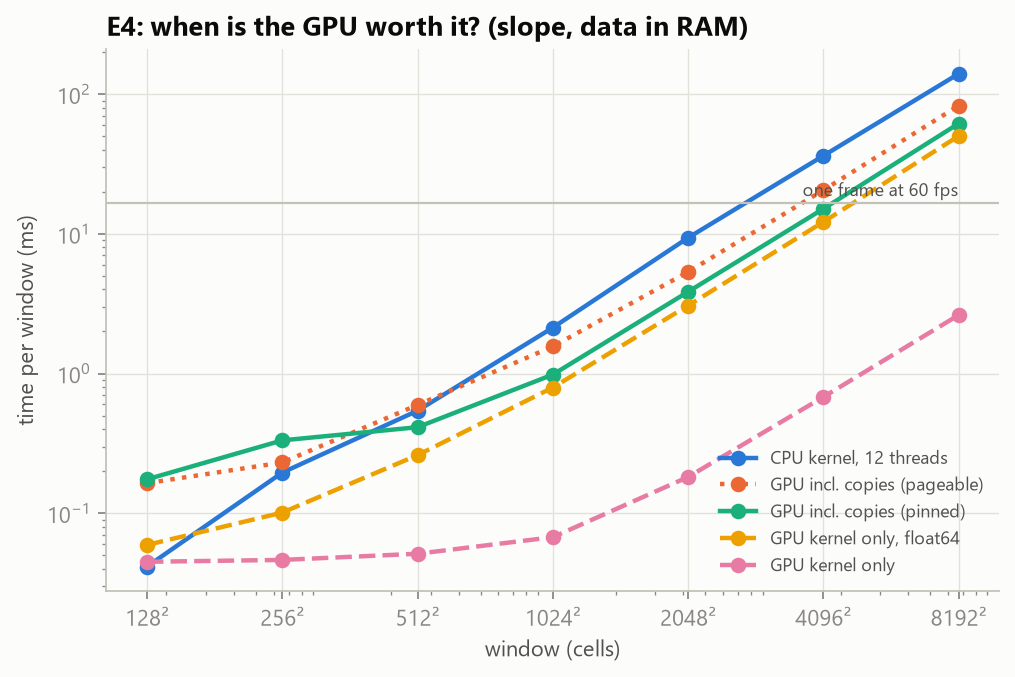
\includegraphics[width=\linewidth]{e4_crossover.png}
\column{0.42\textwidth}
\small
\begin{itemize}
  \item GPU kernel: 1.1\,s for 10.8\,B cells (CPU kernel 34\,s). Whole 1\,m run: \textbf{43.8\,s} vs 60.3\,s.
  \item \alert{Copies are 95\%} of the GPU's own time; the GPU wins only from 512$^2$ cells per window.
  \item Each fix moves the bottleneck: \textbf{compute $\to$ decompress $\to$ write}.
  \item GPU never stressed: $\le$63\,°C, $\le$2\,GiB of 8, no setting changed.
\end{itemize}
\end{columns}
\end{frame}

% ------------------------------------------------------------------ E5
\begin{frame}{E5 (G2): on demand, every tile costs the same at every zoom}
\begin{columns}[T]
\column{0.56\textwidth}
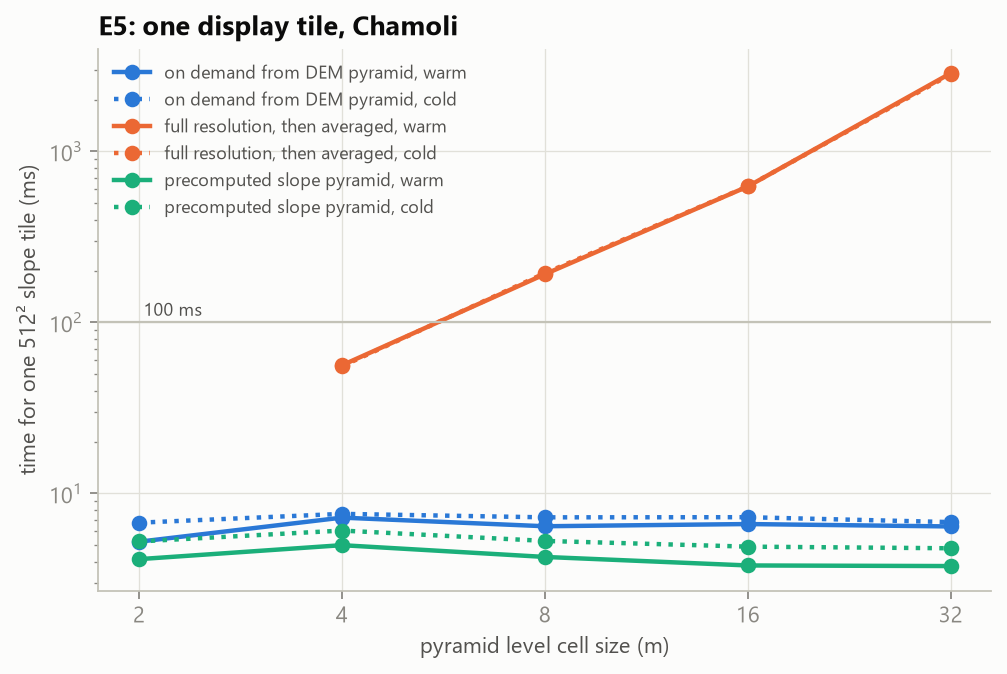
\includegraphics[width=\linewidth]{e5_tile_time.png}
\column{0.42\textwidth}
\begin{itemize}
  \item Slope for a 512$\times$512 tile from pyramid level $k$: \textbf{5--8\,ms} at every level.
  \item Exact (full resolution, then averaged): 56\,ms at 4\,m \ldots\ \textbf{2.9\,s} at 32\,m.
  \item On demand saves \textbf{8--450$\times$}, with \alert{no precomputed storage} (a slope pyramid costs 1.0\,GB
  per derivative).
\end{itemize}
\end{columns}
\end{frame}

\begin{frame}{E5 (G2): the price is slope that is too low}
\begin{columns}[T]
\column{0.5\textwidth}
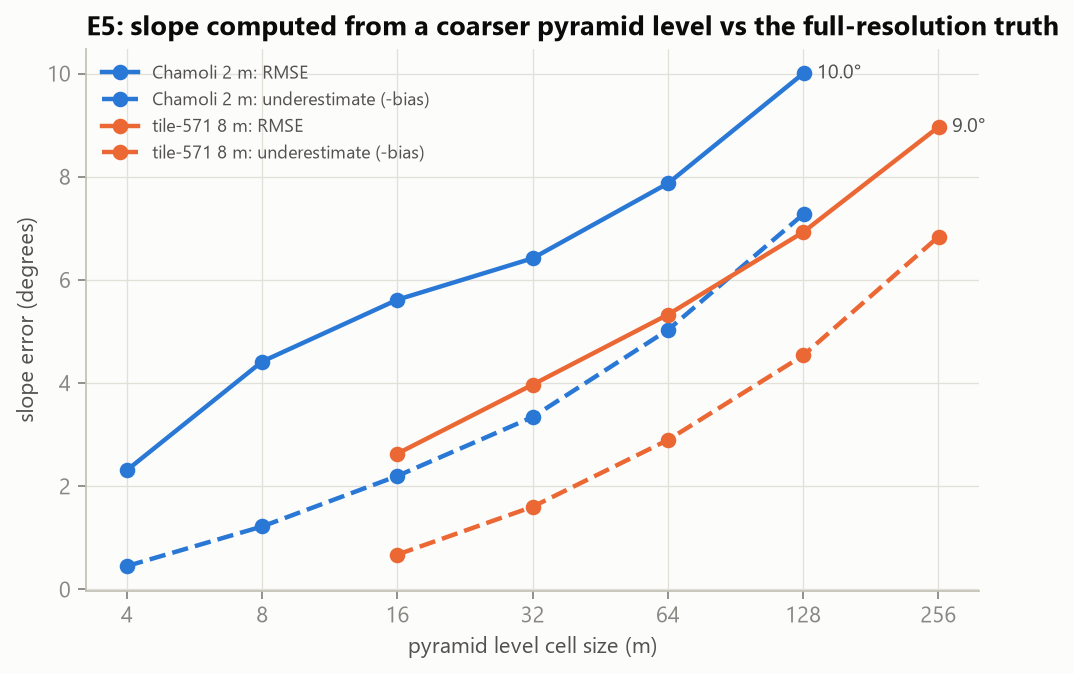
\includegraphics[width=\linewidth]{e5_error_by_level.png}
\column{0.5\textwidth}
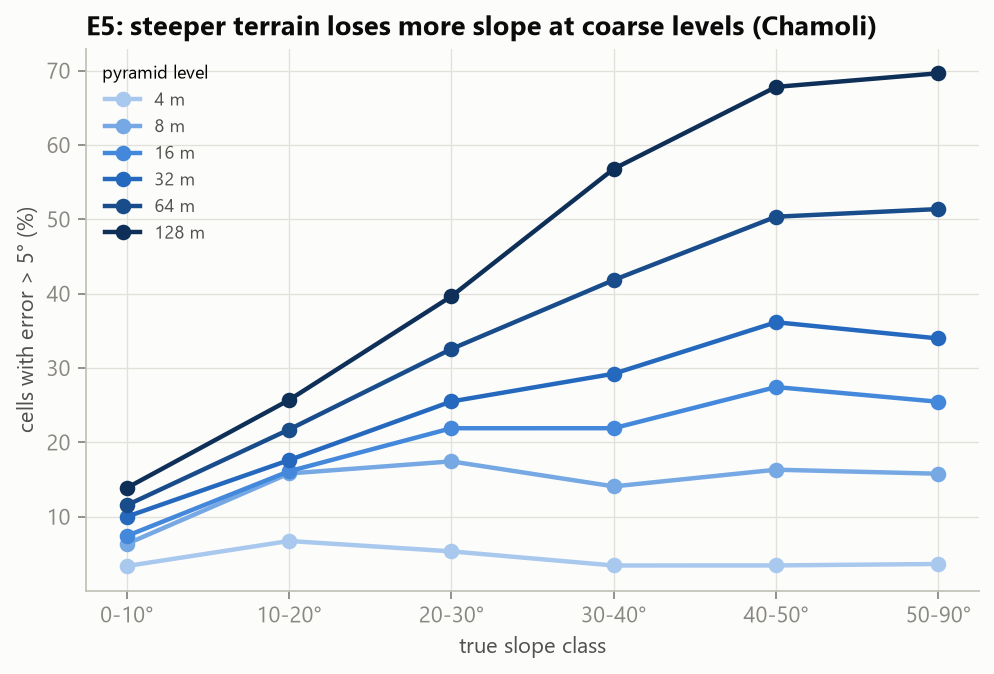
\includegraphics[width=\linewidth]{e5_by_class.png}
\end{columns}
\vspace{2pt}
\small
RMSE (Chamoli 2\,m): \textbf{2.3$^\circ$} one level up $\to$ 6.4$^\circ$ four $\to$ 10.0$^\circ$ six; almost all
\alert{underestimate}, worst on steep ground. Rule of thumb: $\approx$2.5$^\circ$ one level up, +1.5$^\circ$ per
further level. Aspect survives (median 2--8$^\circ$). A pyramid level of good data beats an independent DEM of the
same resolution.
\end{frame}

% ------------------------------------------------------------------ system
\begin{frame}{From findings to a viewer design}
\small
\begin{tabular}{p{0.40\textwidth}p{0.55\textwidth}}
\toprule
Finding & Design decision \\
\midrule
Display needs a pyramid (E1) & Level whose cells fit one screen pixel \\
A tile costs the same at every level (E5) & Fixed 512$^2$ tile lattice per level, aligned to the COG blocks \\
Decoding, not arithmetic, dominates (E3, E5) & Shared cache of decoded blocks; cache of encoded tiles \\
Efficiency cores slow the foreground (E3) & Visible tiles on P-cores, prefetch on E-cores \\
GPU only wins on big windows (E4) & CPU for tiles; GPU left for bulk jobs \\
Coarse levels underestimate slope (E5) & Expected error shown; ``exact'' mode on request \\
\bottomrule
\end{tabular}
\end{frame}

\begin{frame}{The system}
\centering
\resizebox{\linewidth}{!}{%
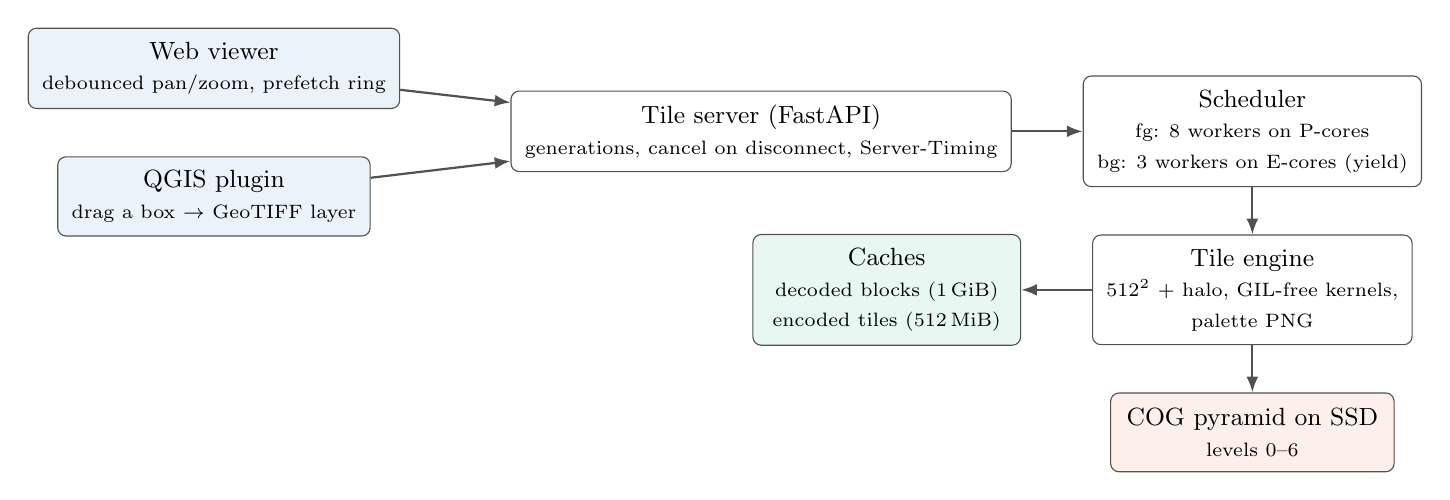
\begin{tikzpicture}[node distance=6mm and 9mm, box/.style={draw=ink2, rounded corners=3pt, align=center,
  font=\small, minimum height=10mm, inner sep=5pt, fill=white}, arr/.style={-{Latex[length=2mm]}, ink2, thick}]
  \node[box, fill=ggblue!10] (web) {Web viewer\\{\scriptsize debounced pan/zoom, prefetch ring}};
  \node[box, fill=ggblue!10, below=of web] (qgis) {QGIS plugin\\{\scriptsize drag a box $\to$ GeoTIFF layer}};
  \node[box, right=14mm of web, yshift=-8mm, minimum width=34mm] (srv) {Tile server (FastAPI)\\{\scriptsize generations,
    cancel on disconnect, Server-Timing}};
  \node[box, right=of srv, minimum width=36mm] (sch) {Scheduler\\{\scriptsize fg: 8 workers on P-cores}\\{\scriptsize
    bg: 3 workers on E-cores (yield)}};
  \node[box, below=of sch, minimum width=36mm] (eng) {Tile engine\\{\scriptsize 512$^2$ + halo, GIL-free kernels,}\\{\scriptsize
    palette PNG}};
  \node[box, left=of eng, minimum width=34mm, fill=gggreen!10] (cache) {Caches\\{\scriptsize decoded blocks (1\,GiB)}\\{\scriptsize
    encoded tiles (512\,MiB)}};
  \node[box, below=of eng, minimum width=36mm, fill=ggorange!10] (cog) {COG pyramid on SSD\\{\scriptsize levels 0--6}};
  \draw[arr] (web) -- (srv); \draw[arr] (qgis) -- (srv); \draw[arr] (srv) -- (sch); \draw[arr] (sch) -- (eng);
  \draw[arr] (eng) -- (cache); \draw[arr] (eng) -- (cog);
\end{tikzpicture}}
\end{frame}

\begin{frame}{How the viewer behaves}
\begin{columns}[T]
\column{0.5\textwidth}
\small
\begin{itemize}
  \item \textbf{Zoom:} every wheel tick moves the camera at once; cached coarser tiles stand in. One
  \alert{commit 150\,ms after the last tick}: new generation, stale requests aborted (the server cancels them).
  \item \textbf{Pan:} newly visible tiles requested immediately.
  \item \textbf{Prefetch:} after a commit, the 8 neighbouring views at low priority, direction of travel first, at
  most 2 in flight; stops at the first input of a gesture.
  \item \textbf{Shift + drag} zooms to a box.
\end{itemize}
\column{0.5\textwidth}
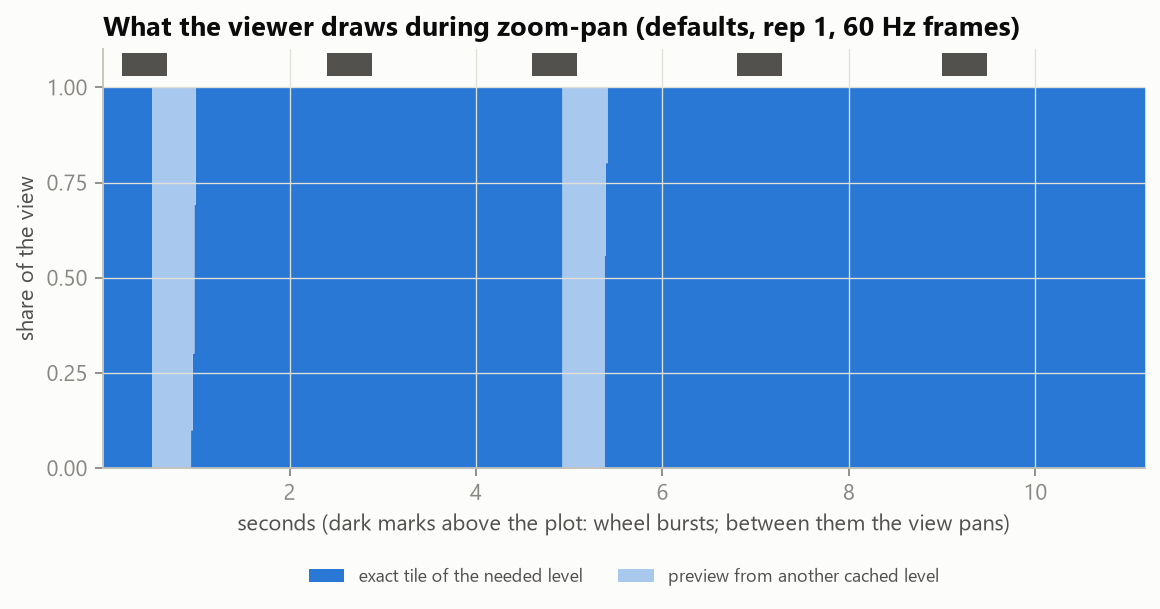
\includegraphics[width=\linewidth]{e6_timeline.png}\\
{\scriptsize Zoom-pan trace: dark = exact tile of the needed level, light = preview from another cached level.}
\end{columns}
\end{frame}

% ------------------------------------------------------------------ E6
\begin{frame}{E6: how we measured the viewer}
\begin{itemize}
  \item \textbf{Virtual client:} the browser's policy ported to Python, reading the same \texttt{policy.json};
  real HTTP, 6 connections like a browser, 60\,Hz frames, aborts close the connection.
  \item \textbf{17 seeded traces:} pans at 0.5/1/2 view widths per second, reversals, random walk, wheel bursts,
  notched wheel, zoom-pan, nested boxes.
  \item \textbf{24 configurations, one factor at a time; 1{,}068 runs}, each on a fresh server (empty caches).
  \item \textbf{Checked against real Chrome} (DevTools protocol): same requests and commits; view-complete within
  10\%.
\end{itemize}
\end{frame}

\begin{frame}{E6: the debounce cuts server work 3.3$\times$}
\begin{columns}[T]
\column{0.62\textwidth}
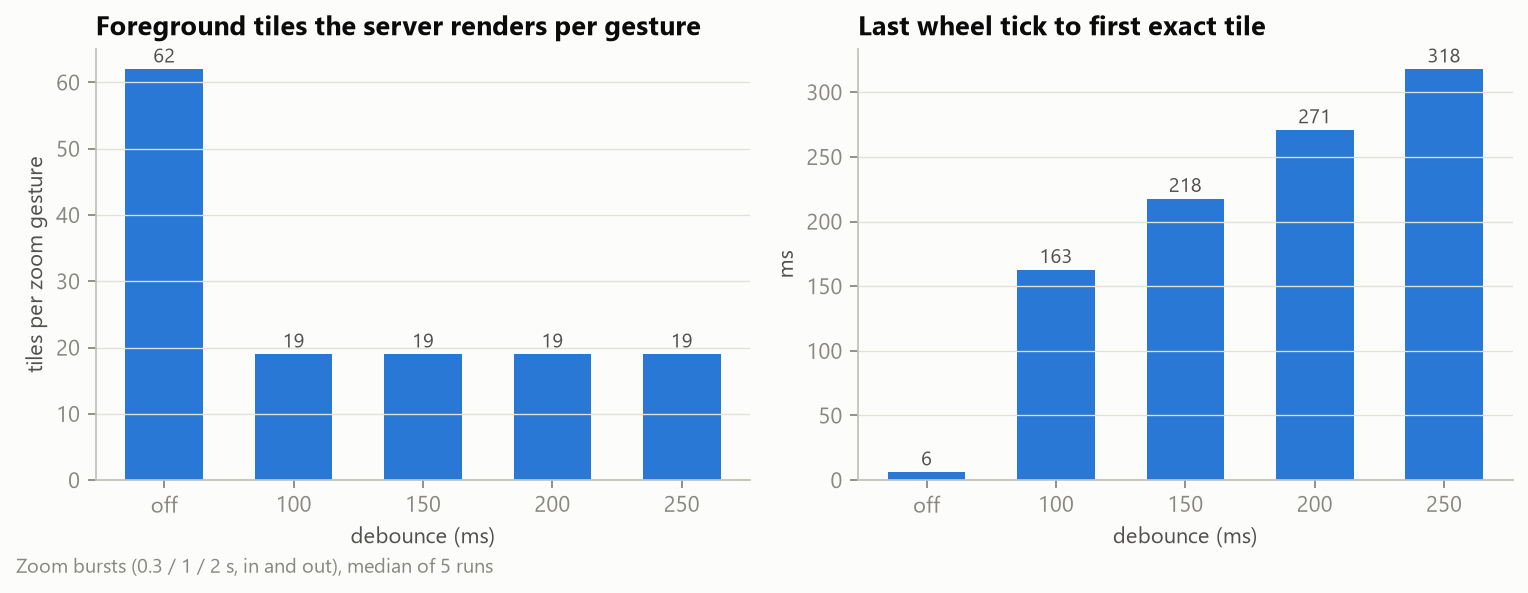
\includegraphics[width=\linewidth]{e6_debounce.png}
\column{0.36\textwidth}
\small
\begin{itemize}
  \item Every tick commits: \textbf{62} server tiles per zoom; debounced: \textbf{19}.
  \item First exact tile \textbf{63--71\,ms} after the debounce (gate: $<$100\,ms).
  \item \textbf{Notched wheel:} 100\,ms = as bad as none (36 tiles); 150\,ms coalesces (15).
  \item $\Rightarrow$ default \alert{150\,ms}.
\end{itemize}
\end{columns}
\end{frame}

\begin{frame}{E6: prefetch makes panning seamless}
\begin{columns}[T]
\column{0.56\textwidth}
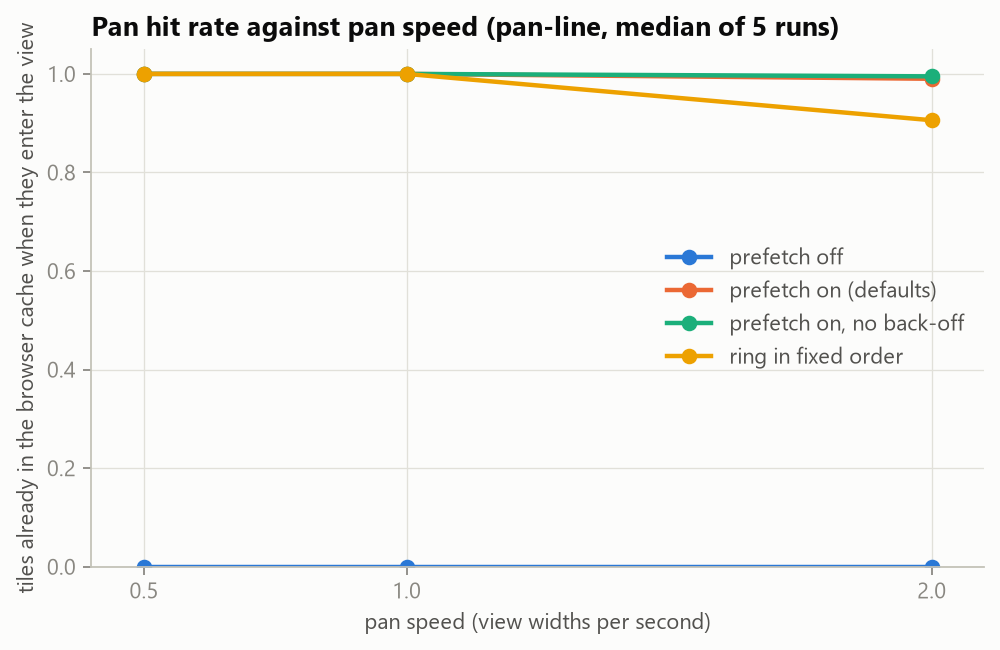
\includegraphics[width=\linewidth]{e6_hit_vs_speed.png}
\column{0.42\textwidth}
\small
\begin{itemize}
  \item After each commit the 8 neighbouring views load at low priority, direction of travel first.
  \item \textbf{98--100\%} of tiles entering the view are already cached, up to 2 view widths per second.
  \item Without prefetch: 0\% on a straight pan, $\sim$50\% when the pan turns back.
  \item Cost: 2--5 tiles fetched per tile used, on the efficiency cores ($\sim$3 CPU-s per 5\,s pan).
\end{itemize}
\end{columns}
\end{frame}

\begin{frame}{E6 gate 1: prefetch does not slow the visible tiles}
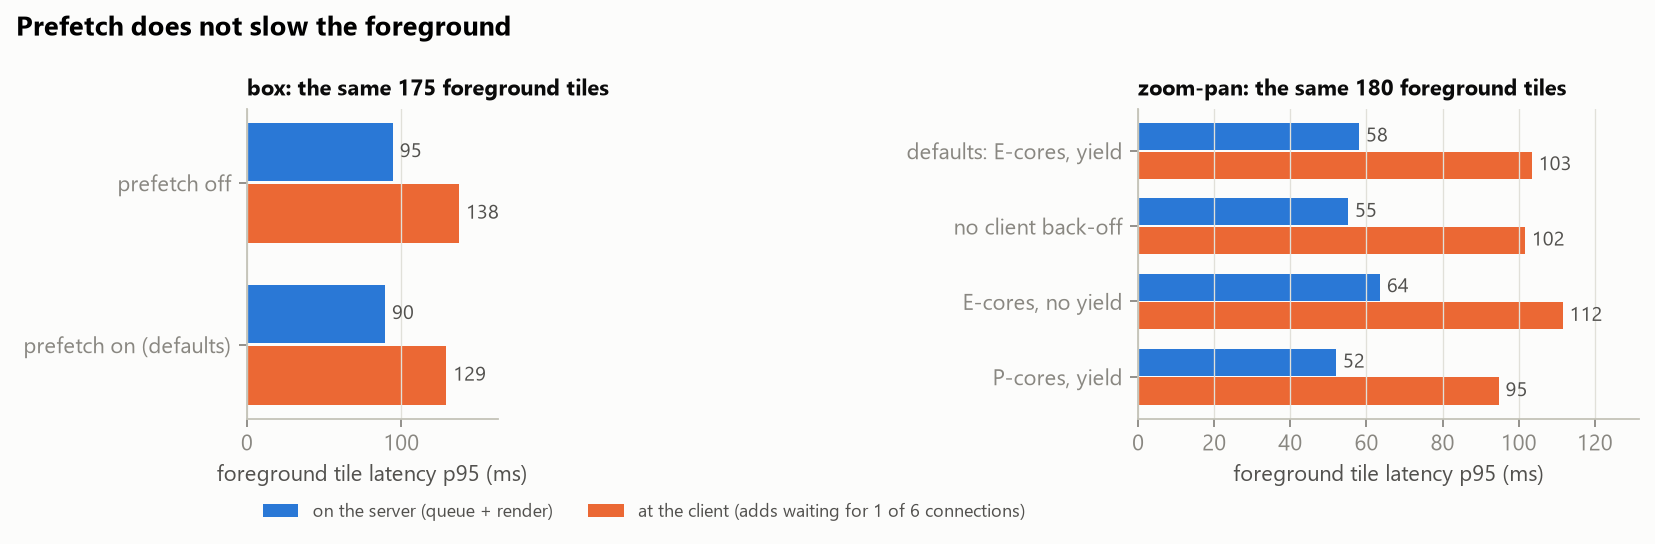
\includegraphics[width=\linewidth]{e6_fg_p95.png}
\small
On identical tiles the server p95 is \textbf{90\,ms with prefetch vs 95\,ms without}: prefetch stops at the first input
of a gesture, so only 3\% of foreground tiles ever overlap it. Every one of 122{,}215 prefetch jobs ran on an
efficiency core.
\end{frame}

\begin{frame}{E6: what sets the remaining latency}
\begin{itemize}
  \item \textbf{The browser's 6 connections:} client p95 $\approx$ server p95 + 40\,ms; 4, 6 or 8 foreground
  workers give the same client latency.
  \item \textbf{Block decoding:} without the block cache, 6$\times$ more blocks decoded and p95 +40\%.
  \item \textbf{Not the derivative:} slope, aspect, hillshade within $\sim$10\%; precomputed slope fastest on the server.
  \item \textbf{Not the disk:} a flushed file cache changes nothing.
  \item A first back-off rule (pause prefetch if foreground p95 $>$ 100\,ms) sat exactly at the cold-start latency and
  switched prefetch off at random; \alert{250\,ms} fixes it.
\end{itemize}
\end{frame}

\begin{frame}{Demo}
\begin{columns}[T]
\column{0.5\textwidth}
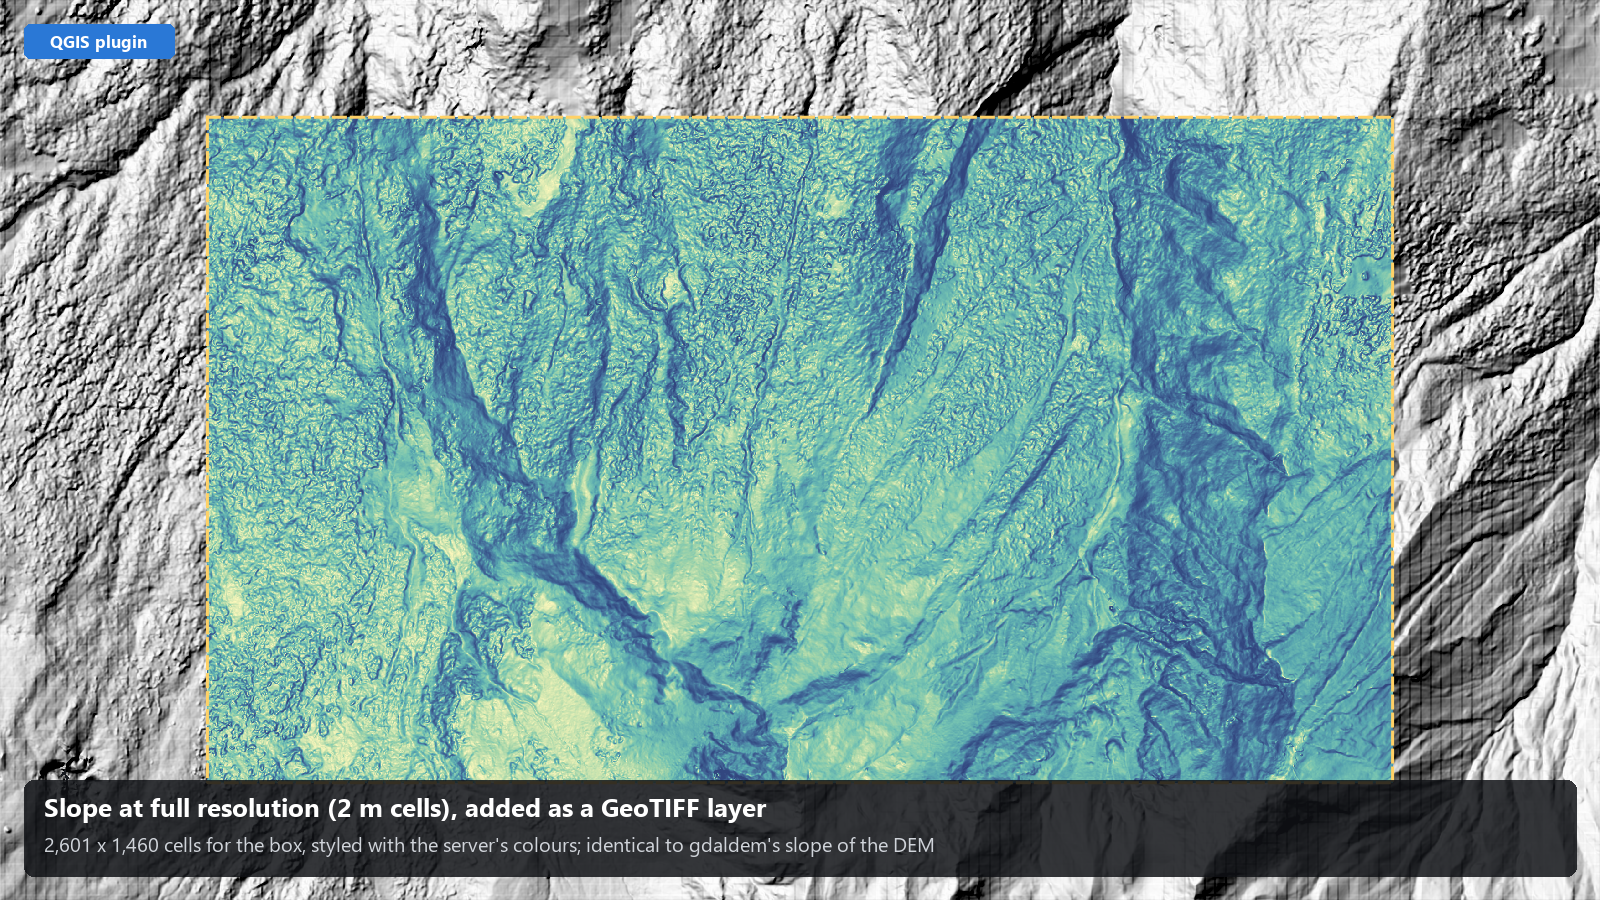
\includegraphics[width=\linewidth]{qgis_q3.png}\\
{\scriptsize QGIS plugin: a 2\,m slope box from the same server.}
\column{0.48\textwidth}
\begin{itemize}
  \item Live: \texttt{python -m server}, then\\ \url{http://127.0.0.1:8765/viewer/}
  \item Wheel zoom, pan, product switch, sun direction, Shift + drag box, status panel (level, cell size, expected
  error)
  \item Fallback video (58\,s):\\ \texttt{report/demo/geoguessers\_demo.mp4}
\end{itemize}
\end{columns}
\end{frame}

% ------------------------------------------------------------------ wrap-up
\begin{frame}{The bottleneck story (G1)}
\centering
\resizebox{\linewidth}{!}{%
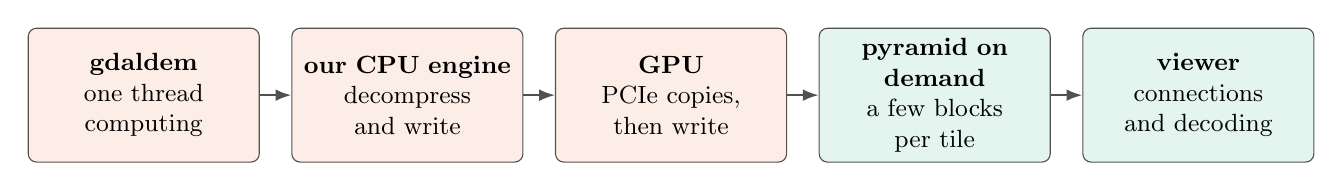
\begin{tikzpicture}[node distance=4mm, st/.style={draw=ink2, rounded corners=3pt, align=center, font=\small,
  text width=27mm, minimum height=17mm, fill=white}, arr/.style={-{Latex[length=2mm]}, ink2, thick}]
  \node[st, fill=ggorange!12] (a) {\textbf{gdaldem}\\one thread\\computing};
  \node[st, right=of a, fill=ggorange!12] (b) {\textbf{our CPU engine}\\decompress\\and write};
  \node[st, right=of b, fill=ggorange!12] (c) {\textbf{GPU}\\PCIe copies,\\then write};
  \node[st, right=of c, fill=gggreen!12] (d) {\textbf{pyramid on demand}\\a few blocks\\per tile};
  \node[st, right=of d, fill=gggreen!12] (e) {\textbf{viewer}\\connections\\and decoding};
  \draw[arr] (a) -- (b); \draw[arr] (b) -- (c); \draw[arr] (c) -- (d); \draw[arr] (d) -- (e);
\end{tikzpicture}}
\vspace{8pt}
\begin{itemize}
  \item On a laptop, standard tools stop being practical by being \textbf{slow, not by running out of memory}.
  \item Once computation is parallel, \alert{moving and decoding data} is the cost; the GPU only shifts it.
  \item Reading \textbf{only what is in view, at the needed level} sidesteps the chain: a tile costs milliseconds at
  any zoom.
\end{itemize}
\end{frame}

\begin{frame}{Limitations and future work}
\begin{columns}[T]
\column{0.5\textwidth}
\textbf{Limitations}
\small
\begin{itemize}
  \item One laptop, one study region (steep terrain: larger slope errors than flat land).
  \item Synthetic 2\,m/1\,m grids used for timing only.
  \item E6: one client, short scripted traces, cold server start.
  \item Coarse-level bias not corrected.
\end{itemize}
\column{0.5\textwidth}
\textbf{Future work}
\small
\begin{itemize}
  \item G3: viewshed (R3 vs XDraw vs \texttt{gdal\_viewshed}) and terrain distance (Dijkstra vs A*).
  \item Per-level slope bias correction.
  \item Several clients and long sessions; remote (cloud) COGs.
  \item GPU tile path for bulk exports; Cesium globe.
\end{itemize}
\end{columns}
\end{frame}

\begin{frame}{Takeaways}
\begin{enumerate}
  \item \textbf{G1:} on one laptop the bottleneck moves from single-threaded computation to decompressing and writing
  data; a GPU computes 50$\times$ faster but the run is only up to 1.4$\times$ faster.
  \item \textbf{G2:} derivatives on demand from the pyramid cost 5--8\,ms per tile at any zoom, 8--450$\times$ less
  than exact, for $\approx$2.5$^\circ$ + 1.5$^\circ$/level slope RMSE (an underestimate).
  \item \textbf{Viewer:} with a 150\,ms debounce and an efficiency-core prefetch ring, on-demand computation keeps up
  with continuous pan and zoom; the browser's connections and block decoding set the latency.
\end{enumerate}
\vspace{8pt}
\centering\small Code, data manifests, results and reports: \url{https://github.com/Swayamgoyal/Geoguessers}
\end{frame}

\begin{frame}[plain]
\vfill\centering{\Huge\bfseries Thank you}\\[10pt]{\Large\color{ggblue} Questions?}\vfill
\end{frame}

\end{document}
